% !Rnw root = learnR.Rnw

%% ---preamble.tex----%% 
%% maxwidth is the original width if it is less than linewidth
%% otherwise use linewidth (to make sure the graphics do not exceed the margin)
\makeatletter
\def\maxwidth{ %
  \ifdim\Gin@nat@width>\linewidth
    \linewidth
  \else
    \Gin@nat@width
  \fi
}
\makeatother

\definecolor{fgcolor}{rgb}{0.345, 0.345, 0.345}

\definecolor{shadecolor}{rgb}{.97, .97, .97}
\definecolor{messagecolor}{rgb}{0, 0, 0}
\definecolor{warningcolor}{rgb}{1, 0, 1}
\definecolor{errorcolor}{rgb}{1, 0, 0}






These graphs are included separately because they benefit from
explanatory annotation and/or do require color to be effective.

\subsection*{Annotated Motion Chart}

\begin{figure*}[h]
\vspace*{-6pt}
\centerline{\includegraphics[scale=0.88]{colorArt/motionchart}}%
\caption{Snapshot of a motion chart, with annotation
  that identifies selected chart features that can be
  modified interactively.\label{col:mchart}}
\vspace*{-18pt}
\end{figure*}

\newpage
\subsection*{Florence Nightingale's Wedge Plot}\label{sec:wedge}

\marginnote[-24pt]{The name `coxcomb' arose from a misreading of
  Florence Nightingale's \textit{Mortality of the British Army} that
  was an annex to a larger official report. See {\small
    \url{http://www.york.ac.uk/depts/maths/histstat/small.htm}}}

Figure \ref{col:wedgeplot} is a `wedge' plot that shows the
mortality of British troops according to cause in the Crimean War over
1853-1853. It has often been called a `coxcomb' plot -- a name that
suits this imaginative form of graphical presentation.

\begin{figure*}
\centerline{\includegraphics[width=0.97\textwidth]{colorArt/allwedge}}%
\caption{Deaths (per 1000 per annum), up to and after the
  Sanitary Commission's visit in March 1855.  Areas, measured from the
centres of the common vertices, are proportional
  to mortalities..\label{col:wedgeplot}}
\end{figure*}

Figure \ref{col:wedgeplot} is used here to show abilities in
\textit{ggplot2}.  The wedge plot is not ideal for giving an accurate
sense of the data.  It is not however easy to suggest an alternative
that is clearly better.

\subsection*{ Code for the wedge plot}

The url
\url{http://maths-people.anu.edu.au/~johnm/r/functions/wedgeORbubble.R}.\sidenote[][-1cm]{Data
  are from the data frame \txtt{Nightingale} in the {\em HistData}
  package. Subsection \ref{col:wedgeplot} showed how to create a
  dataset \txtt{Crimean} that is in a convenient form for creating
  this plot.} has code for the function \txtt{wedgeplot()} that was
used for this plot.  Note also the function \txtt{gdot()} that
gives a not entirely satisfactory alternative to the wedge plot.

\newpage
\subsection*{Selected base graphics parameter settings}
\enlargethispage{12pt}
\begin{figure*}
\vspace*{-10pt}

\centerline{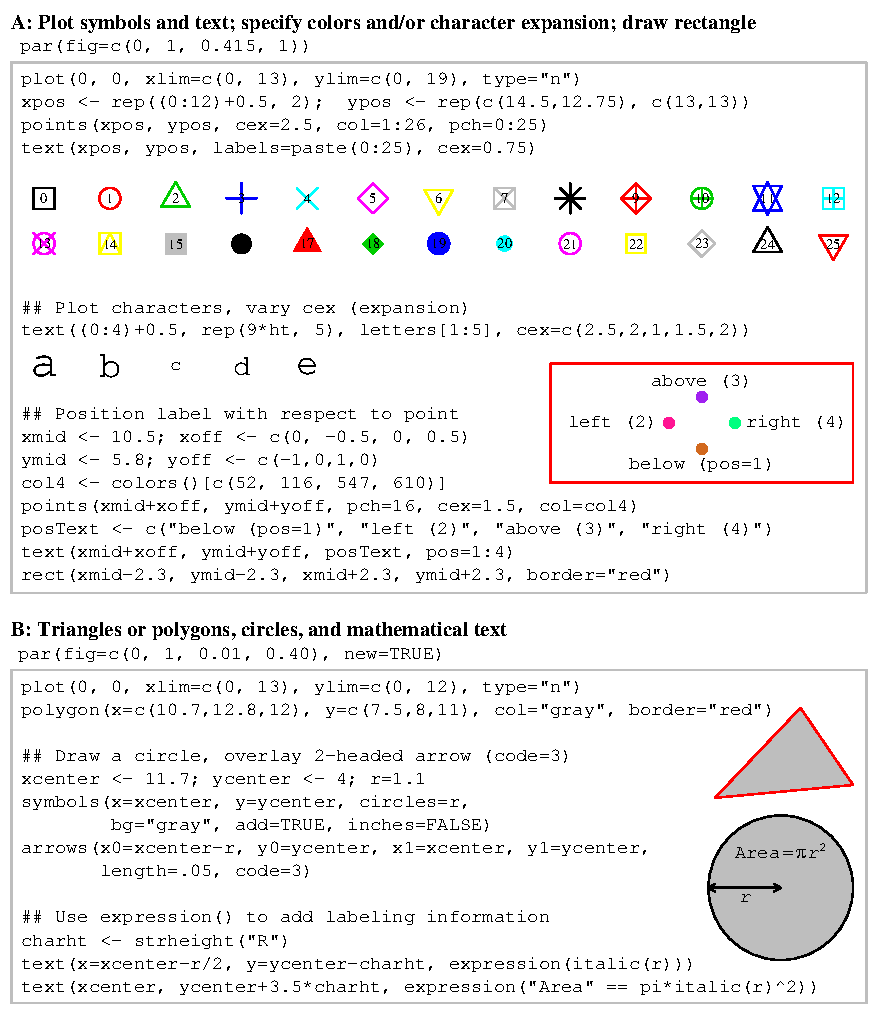
\includegraphics[width=0.875\textwidth]{colorArt/gphpars}}

\caption{Here are demonstrated selected parameter settings and
abilities that relate to Section \ref{ss:fine}.\label{fig:pars}}.
\end{figure*}

%
% \begin{fullwidth}
% Note that the function \texttt{paste()}, used in line 5 of Panel A, 
% turns the
%   vector of numerical values \texttt{0:12} into a vector of character
%   strings with elements \texttt{"0", "1", ..., "12"}.  An alternative to
% \texttt{paste(0:12)} is \texttt{as.character(0:12)}.
% \end{fullwidth}
\vfill
